\documentclass[1p]{elsarticle_modified}
%\bibliographystyle{elsarticle-num}

%\usepackage[colorlinks]{hyperref}
%\usepackage{abbrmath_seonhwa} %\Abb, \Ascr, \Acal ,\Abf, \Afrak
\usepackage{amsfonts}
\usepackage{amssymb}
\usepackage{amsmath}
\usepackage{amsthm}
\usepackage{scalefnt}
\usepackage{amsbsy}
\usepackage{kotex}
\usepackage{caption}
\usepackage{subfig}
\usepackage{color}
\usepackage{graphicx}
\usepackage{xcolor} %% white, black, red, green, blue, cyan, magenta, yellow
\usepackage{float}
\usepackage{setspace}
\usepackage{hyperref}

\usepackage{tikz}
\usetikzlibrary{arrows}

\usepackage{multirow}
\usepackage{array} % fixed length table
\usepackage{hhline}

%%%%%%%%%%%%%%%%%%%%%
\makeatletter
\renewcommand*\env@matrix[1][\arraystretch]{%
	\edef\arraystretch{#1}%
	\hskip -\arraycolsep
	\let\@ifnextchar\new@ifnextchar
	\array{*\c@MaxMatrixCols c}}
\makeatother %https://tex.stackexchange.com/questions/14071/how-can-i-increase-the-line-spacing-in-a-matrix
%%%%%%%%%%%%%%%

\usepackage[normalem]{ulem}

\newcommand{\msout}[1]{\ifmmode\text{\sout{\ensuremath{#1}}}\else\sout{#1}\fi}
%SOURCE: \msout is \stkout macro in https://tex.stackexchange.com/questions/20609/strikeout-in-math-mode

\newcommand{\cancel}[1]{
	\ifmmode
	{\color{red}\msout{#1}}
	\else
	{\color{red}\sout{#1}}
	\fi
}

\newcommand{\add}[1]{
	{\color{blue}\uwave{#1}}
}

\newcommand{\replace}[2]{
	\ifmmode
	{\color{red}\msout{#1}}{\color{blue}\uwave{#2}}
	\else
	{\color{red}\sout{#1}}{\color{blue}\uwave{#2}}
	\fi
}

\newcommand{\Sol}{\mathcal{S}} %segment
\newcommand{\D}{D} %diagram
\newcommand{\A}{\mathcal{A}} %arc


%%%%%%%%%%%%%%%%%%%%%%%%%%%%%5 test

\def\sl{\operatorname{\textup{SL}}(2,\Cbb)}
\def\psl{\operatorname{\textup{PSL}}(2,\Cbb)}
\def\quan{\mkern 1mu \triangleright \mkern 1mu}

\theoremstyle{definition}
\newtheorem{thm}{Theorem}[section]
\newtheorem{prop}[thm]{Proposition}
\newtheorem{lem}[thm]{Lemma}
\newtheorem{ques}[thm]{Question}
\newtheorem{cor}[thm]{Corollary}
\newtheorem{defn}[thm]{Definition}
\newtheorem{exam}[thm]{Example}
\newtheorem{rmk}[thm]{Remark}
\newtheorem{alg}[thm]{Algorithm}

\newcommand{\I}{\sqrt{-1}}
\begin{document}

%\begin{frontmatter}
%
%\title{Boundary parabolic representations of knots up to 8 crossings}
%
%%% Group authors per affiliation:
%\author{Yunhi Cho} 
%\address{Department of Mathematics, University of Seoul, Seoul, Korea}
%\ead{yhcho@uos.ac.kr}
%
%
%\author{Seonhwa Kim} %\fnref{s_kim}}
%\address{Center for Geometry and Physics, Institute for Basic Science, Pohang, 37673, Korea}
%\ead{ryeona17@ibs.re.kr}
%
%\author{Hyuk Kim}
%\address{Department of Mathematical Sciences, Seoul National University, Seoul 08826, Korea}
%\ead{hyukkim@snu.ac.kr}
%
%\author{Seokbeom Yoon}
%\address{Department of Mathematical Sciences, Seoul National University, Seoul, 08826,  Korea}
%\ead{sbyoon15@snu.ac.kr}
%
%\begin{abstract}
%We find all boundary parabolic representation of knots up to 8 crossings.
%
%\end{abstract}
%\begin{keyword}
%    \MSC[2010] 57M25 
%\end{keyword}
%
%\end{frontmatter}

%\linenumbers
%\tableofcontents
%
\newcommand\colored[1]{\textcolor{white}{\rule[-0.35ex]{0.8em}{1.4ex}}\kern-0.8em\color{red} #1}%
%\newcommand\colored[1]{\textcolor{white}{ #1}\kern-2.17ex	\textcolor{white}{ #1}\kern-1.81ex	\textcolor{white}{ #1}\kern-2.15ex\color{red}#1	}

{\Large $\underline{12a_{1223}~(K12a_{1223})}$}

\setlength{\tabcolsep}{10pt}
\renewcommand{\arraystretch}{1.6}
\vspace{1cm}\begin{tabular}{m{100pt}>{\centering\arraybackslash}m{274pt}}
\multirow{5}{120pt}{
	\centering
	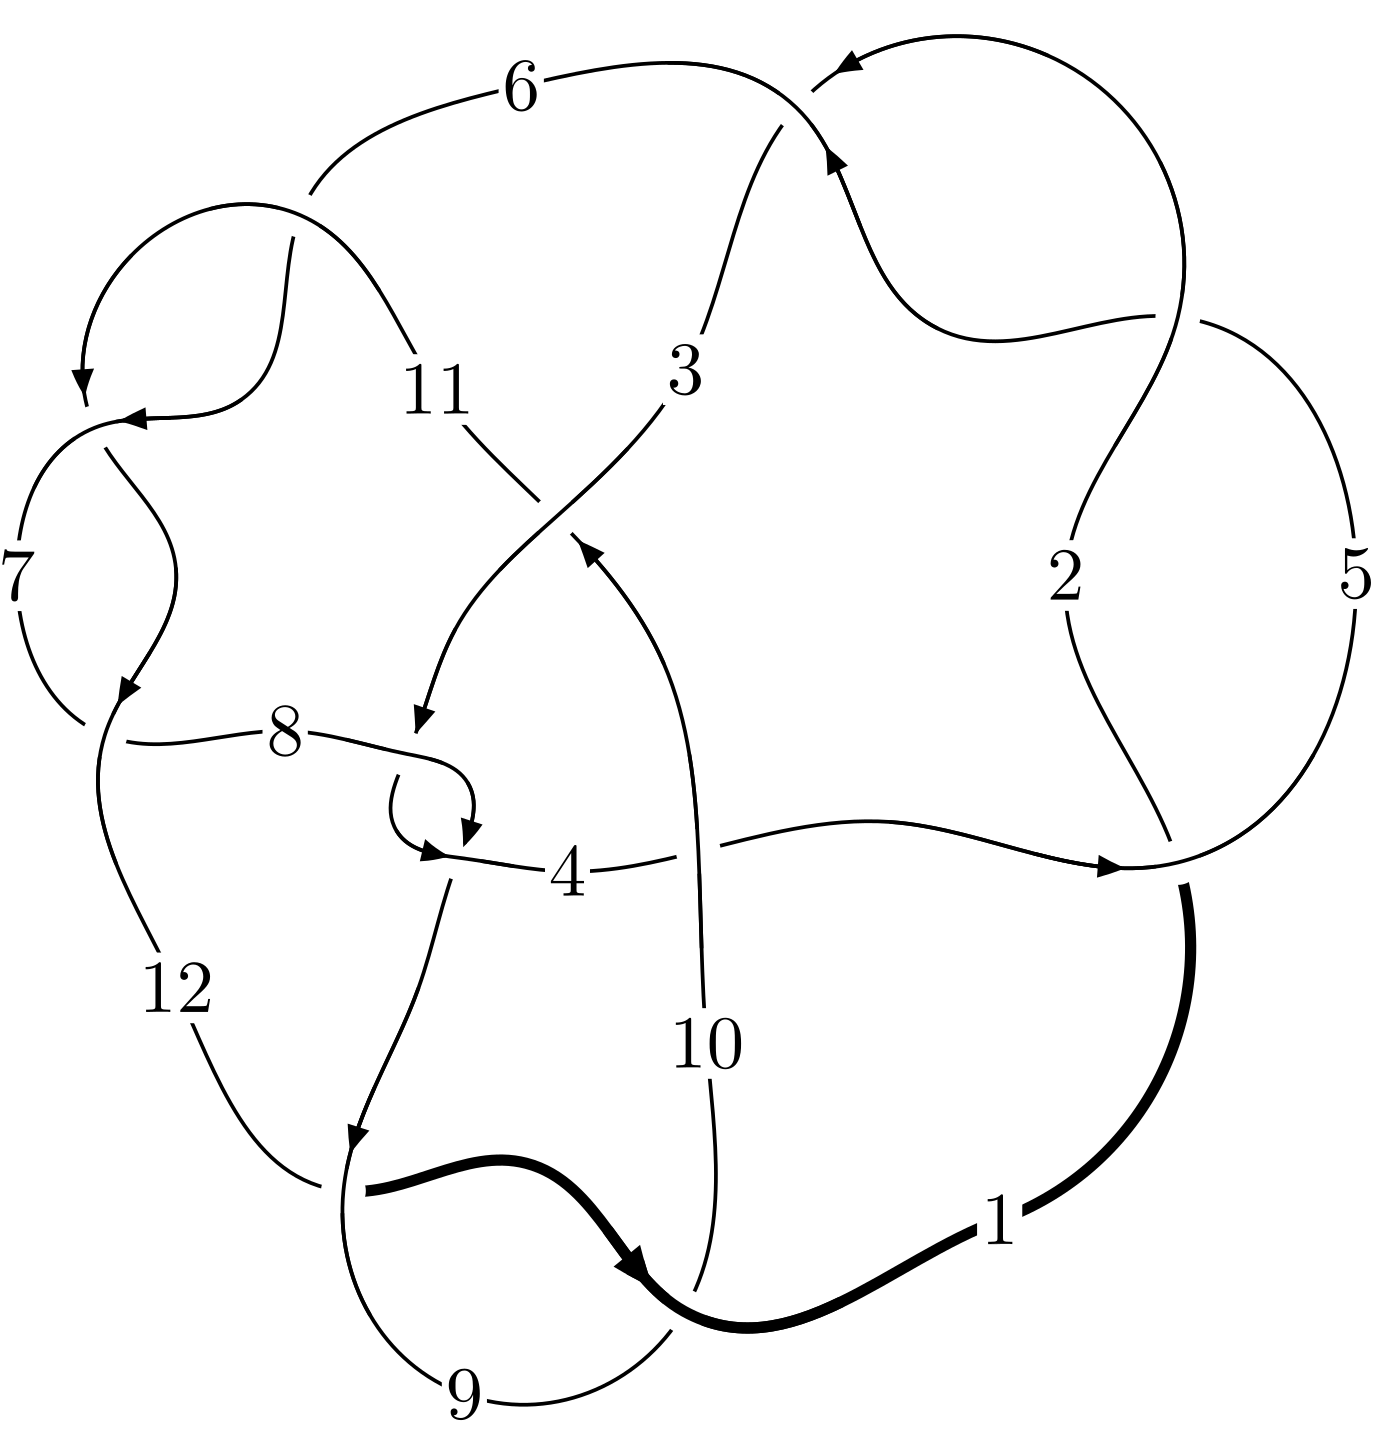
\includegraphics[width=112pt]{../../../GIT/diagram.site/Diagrams/png/2024_12a_1223.png}\\
\ \ \ A knot diagram\footnotemark}&
\allowdisplaybreaks
\textbf{Linearized knot diagam} \\
\cline{2-2}
 &
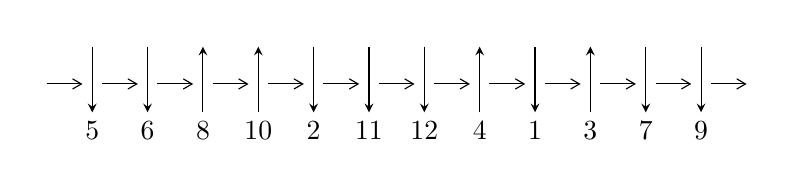
\begin{tikzpicture}[x=20pt, y=17pt]
	% nodes
	\node (C0) at (0, 0) {};
	\node (C1) at (1, 0) {};
	\node (C1U) at (1, +1) {};
	\node (C1D) at (1, -1) {5};

	\node (C2) at (2, 0) {};
	\node (C2U) at (2, +1) {};
	\node (C2D) at (2, -1) {6};

	\node (C3) at (3, 0) {};
	\node (C3U) at (3, +1) {};
	\node (C3D) at (3, -1) {8};

	\node (C4) at (4, 0) {};
	\node (C4U) at (4, +1) {};
	\node (C4D) at (4, -1) {10};

	\node (C5) at (5, 0) {};
	\node (C5U) at (5, +1) {};
	\node (C5D) at (5, -1) {2};

	\node (C6) at (6, 0) {};
	\node (C6U) at (6, +1) {};
	\node (C6D) at (6, -1) {11};

	\node (C7) at (7, 0) {};
	\node (C7U) at (7, +1) {};
	\node (C7D) at (7, -1) {12};

	\node (C8) at (8, 0) {};
	\node (C8U) at (8, +1) {};
	\node (C8D) at (8, -1) {4};

	\node (C9) at (9, 0) {};
	\node (C9U) at (9, +1) {};
	\node (C9D) at (9, -1) {1};

	\node (C10) at (10, 0) {};
	\node (C10U) at (10, +1) {};
	\node (C10D) at (10, -1) {3};

	\node (C11) at (11, 0) {};
	\node (C11U) at (11, +1) {};
	\node (C11D) at (11, -1) {7};

	\node (C12) at (12, 0) {};
	\node (C12U) at (12, +1) {};
	\node (C12D) at (12, -1) {9};
	\node (C13) at (13, 0) {};

	% arrows
	\draw[->,>={angle 60}]
	(C0) edge (C1) (C1) edge (C2) (C2) edge (C3) (C3) edge (C4) (C4) edge (C5) (C5) edge (C6) (C6) edge (C7) (C7) edge (C8) (C8) edge (C9) (C9) edge (C10) (C10) edge (C11) (C11) edge (C12) (C12) edge (C13) ;	\draw[->,>=stealth]
	(C1U) edge (C1D) (C2U) edge (C2D) (C3D) edge (C3U) (C4D) edge (C4U) (C5U) edge (C5D) (C6U) edge (C6D) (C7U) edge (C7D) (C8D) edge (C8U) (C9U) edge (C9D) (C10D) edge (C10U) (C11U) edge (C11D) (C12U) edge (C12D) ;
	\end{tikzpicture} \\
\hhline{~~} \\& 
\textbf{Solving Sequence} \\ \cline{2-2} 
 &
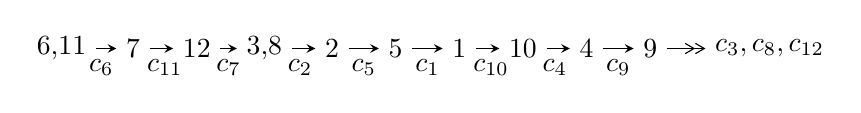
\begin{tikzpicture}[x=23pt, y=7pt]
	% node
	\node (A0) at (-1/8, 0) {6,11};
	\node (A1) at (1, 0) {7};
	\node (A2) at (2, 0) {12};
	\node (A3) at (49/16, 0) {3,8};
	\node (A4) at (33/8, 0) {2};
	\node (A5) at (41/8, 0) {5};
	\node (A6) at (49/8, 0) {1};
	\node (A7) at (57/8, 0) {10};
	\node (A8) at (65/8, 0) {4};
	\node (A9) at (73/8, 0) {9};
	\node (C1) at (1/2, -1) {$c_{6}$};
	\node (C2) at (3/2, -1) {$c_{11}$};
	\node (C3) at (5/2, -1) {$c_{7}$};
	\node (C4) at (29/8, -1) {$c_{2}$};
	\node (C5) at (37/8, -1) {$c_{5}$};
	\node (C6) at (45/8, -1) {$c_{1}$};
	\node (C7) at (53/8, -1) {$c_{10}$};
	\node (C8) at (61/8, -1) {$c_{4}$};
	\node (C9) at (69/8, -1) {$c_{9}$};
	\node (A10) at (11, 0) {$c_{3},c_{8},c_{12}$};

	% edge
	\draw[->,>=stealth]	
	(A0) edge (A1) (A1) edge (A2) (A2) edge (A3) (A3) edge (A4) (A4) edge (A5) (A5) edge (A6) (A6) edge (A7) (A7) edge (A8) (A8) edge (A9) ;
	\draw[->>,>={angle 60}]	
	(A9) edge (A10);
\end{tikzpicture} \\ 

\end{tabular} \\

\footnotetext{
The image of knot diagram is generated by the software ``\textbf{Draw programme}" developed by Andrew Bartholomew(\url{http://www.layer8.co.uk/maths/draw/index.htm\#Running-draw}), where we modified some parts for our purpose(\url{https://github.com/CATsTAILs/LinksPainter}).
}\phantom \\ \newline 
\centering \textbf{Ideals for irreducible components\footnotemark of $X_{\text{par}}$} 
 
\begin{align*}
I^u_{1}&=\langle 
3.57598\times10^{170} u^{85}+1.01646\times10^{170} u^{84}+\cdots+2.31147\times10^{171} b-4.59337\times10^{171},\\
\phantom{I^u_{1}}&\phantom{= \langle  }8.19062\times10^{171} u^{85}+1.94837\times10^{172} u^{84}+\cdots+1.61803\times10^{172} a-2.37902\times10^{173},\;u^{86}+2 u^{85}+\cdots-43 u-7\rangle \\
I^u_{2}&=\langle 
u^7-4 u^5+u^4+4 u^3-2 u^2+b+1,\\
\phantom{I^u_{2}}&\phantom{= \langle  }u^{15}-9 u^{13}+2 u^{12}+31 u^{11}-14 u^{10}-48 u^9+36 u^8+26 u^7-40 u^6+8 u^5+16 u^4-8 u^3+a,\\
\phantom{I^u_{2}}&\phantom{= \langle  }u^{18}- u^{17}+\cdots- u+1\rangle \\
\\
\end{align*}
\raggedright * 2 irreducible components of $\dim_{\mathbb{C}}=0$, with total 104 representations.\\
\footnotetext{All coefficients of polynomials are rational numbers. But the coefficients are sometimes approximated in decimal forms when there is not enough margin.}
\newpage
\renewcommand{\arraystretch}{1}
\centering \section*{I. $I^u_{1}= \langle 3.58\times10^{170} u^{85}+1.02\times10^{170} u^{84}+\cdots+2.31\times10^{171} b-4.59\times10^{171},\;8.19\times10^{171} u^{85}+1.95\times10^{172} u^{84}+\cdots+1.62\times10^{172} a-2.38\times10^{173},\;u^{86}+2 u^{85}+\cdots-43 u-7 \rangle$}
\flushleft \textbf{(i) Arc colorings}\\
\begin{tabular}{m{7pt} m{180pt} m{7pt} m{180pt} }
\flushright $a_{6}=$&$\begin{pmatrix}1\\0\end{pmatrix}$ \\
\flushright $a_{11}=$&$\begin{pmatrix}0\\u\end{pmatrix}$ \\
\flushright $a_{7}=$&$\begin{pmatrix}1\\u^2\end{pmatrix}$ \\
\flushright $a_{12}=$&$\begin{pmatrix}- u\\- u^3+u\end{pmatrix}$ \\
\flushright $a_{3}=$&$\begin{pmatrix}-0.506210 u^{85}-1.20416 u^{84}+\cdots+19.3397 u+14.7032\\-0.154706 u^{85}-0.0439746 u^{84}+\cdots+0.0924782 u+1.98721\end{pmatrix}$ \\
\flushright $a_{8}=$&$\begin{pmatrix}- u^2+1\\- u^4+2 u^2\end{pmatrix}$ \\
\flushright $a_{2}=$&$\begin{pmatrix}-0.660916 u^{85}-1.24814 u^{84}+\cdots+19.4322 u+16.6904\\-0.154706 u^{85}-0.0439746 u^{84}+\cdots+0.0924782 u+1.98721\end{pmatrix}$ \\
\flushright $a_{5}=$&$\begin{pmatrix}0.0356140 u^{85}+0.948982 u^{84}+\cdots-85.0217 u-27.4994\\-1.04716 u^{85}-0.439822 u^{84}+\cdots+37.0962 u+3.37904\end{pmatrix}$ \\
\flushright $a_{1}=$&$\begin{pmatrix}3.18148 u^{85}+2.79945 u^{84}+\cdots-96.9770 u-29.8437\\2.86152 u^{85}+1.39695 u^{84}+\cdots-91.4443 u-18.0567\end{pmatrix}$ \\
\flushright $a_{10}=$&$\begin{pmatrix}-0.994047 u^{85}-1.13219 u^{84}+\cdots+98.6363 u+6.28721\\-0.776751 u^{85}-0.662827 u^{84}+\cdots+15.6810 u+7.57944\end{pmatrix}$ \\
\flushright $a_{4}=$&$\begin{pmatrix}-1.04225 u^{85}-1.40402 u^{84}+\cdots+33.9514 u+17.8765\\-0.397611 u^{85}-0.156340 u^{84}+\cdots+6.69560 u+3.09603\end{pmatrix}$ \\
\flushright $a_{9}=$&$\begin{pmatrix}2.45518 u^{85}+1.64740 u^{84}+\cdots-104.010 u-27.7858\\2.48561 u^{85}+1.37154 u^{84}+\cdots-43.7893 u-10.0526\end{pmatrix}$\\&\end{tabular}
\flushleft \textbf{(ii) Obstruction class $= -1$}\\~\\
\flushleft \textbf{(iii) Cusp Shapes $= 0.959329 u^{85}-0.908484 u^{84}+\cdots-101.771 u-16.8438$}\\~\\
\newpage\renewcommand{\arraystretch}{1}
\flushleft \textbf{(iv) u-Polynomials at the component}\newline \\
\begin{tabular}{m{50pt}|m{274pt}}
Crossings & \hspace{64pt}u-Polynomials at each crossing \\
\hline $$\begin{aligned}c_{1},c_{2},c_{5}\end{aligned}$$&$\begin{aligned}
&u^{86}+6 u^{85}+\cdots-158 u+47
\end{aligned}$\\
\hline $$\begin{aligned}c_{3},c_{8}\end{aligned}$$&$\begin{aligned}
&u^{86}-24 u^{84}+\cdots+2 u+1
\end{aligned}$\\
\hline $$\begin{aligned}c_{4}\end{aligned}$$&$\begin{aligned}
&u^{86}- u^{85}+\cdots-33283 u+13877
\end{aligned}$\\
\hline $$\begin{aligned}c_{6},c_{7},c_{11}\end{aligned}$$&$\begin{aligned}
&u^{86}-2 u^{85}+\cdots+43 u-7
\end{aligned}$\\
\hline $$\begin{aligned}c_{9},c_{12}\end{aligned}$$&$\begin{aligned}
&u^{86}-2 u^{85}+\cdots+46 u-1
\end{aligned}$\\
\hline $$\begin{aligned}c_{10}\end{aligned}$$&$\begin{aligned}
&u^{86}+3 u^{85}+\cdots+1643283 u+1221183
\end{aligned}$\\
\hline
\end{tabular}\\~\\
\newpage\renewcommand{\arraystretch}{1}
\flushleft \textbf{(v) Riley Polynomials at the component}\newline \\
\begin{tabular}{m{50pt}|m{274pt}}
Crossings & \hspace{64pt}Riley Polynomials at each crossing \\
\hline $$\begin{aligned}c_{1},c_{2},c_{5}\end{aligned}$$&$\begin{aligned}
&y^{86}-100 y^{85}+\cdots-128552 y+2209
\end{aligned}$\\
\hline $$\begin{aligned}c_{3},c_{8}\end{aligned}$$&$\begin{aligned}
&y^{86}-48 y^{85}+\cdots-36 y+1
\end{aligned}$\\
\hline $$\begin{aligned}c_{4}\end{aligned}$$&$\begin{aligned}
&y^{86}+33 y^{85}+\cdots-67871217 y+192571129
\end{aligned}$\\
\hline $$\begin{aligned}c_{6},c_{7},c_{11}\end{aligned}$$&$\begin{aligned}
&y^{86}-92 y^{85}+\cdots-3039 y+49
\end{aligned}$\\
\hline $$\begin{aligned}c_{9},c_{12}\end{aligned}$$&$\begin{aligned}
&y^{86}-72 y^{85}+\cdots-8784 y+1
\end{aligned}$\\
\hline $$\begin{aligned}c_{10}\end{aligned}$$&$\begin{aligned}
&y^{86}+45 y^{85}+\cdots+22828629889629 y+1491287919489
\end{aligned}$\\
\hline
\end{tabular}\\~\\
\newpage\flushleft \textbf{(vi) Complex Volumes and Cusp Shapes}
$$\begin{array}{c|c|c}  
\text{Solutions to }I^u_{1}& \I (\text{vol} + \sqrt{-1}CS) & \text{Cusp shape}\\
 \hline 
\begin{aligned}
u &= -0.789217 + 0.531072 I \\
a &= -0.333546 + 1.319880 I \\
b &= \phantom{-}1.57228 - 0.20818 I\end{aligned}
 & -10.78230 + 6.15211 I & \phantom{-0.000000 } 0 \\ \hline\begin{aligned}
u &= -0.789217 - 0.531072 I \\
a &= -0.333546 - 1.319880 I \\
b &= \phantom{-}1.57228 + 0.20818 I\end{aligned}
 & -10.78230 - 6.15211 I & \phantom{-0.000000 } 0 \\ \hline\begin{aligned}
u &= \phantom{-}0.504496 + 0.785795 I \\
a &= -0.224964 - 1.153010 I \\
b &= \phantom{-}0.630992 + 0.646745 I\end{aligned}
 & -0.62218 - 8.31784 I & \phantom{-0.000000 } 0 \\ \hline\begin{aligned}
u &= \phantom{-}0.504496 - 0.785795 I \\
a &= -0.224964 + 1.153010 I \\
b &= \phantom{-}0.630992 - 0.646745 I\end{aligned}
 & -0.62218 + 8.31784 I & \phantom{-0.000000 } 0 \\ \hline\begin{aligned}
u &= \phantom{-}0.693135 + 0.815814 I \\
a &= -0.560371 + 0.113537 I \\
b &= \phantom{-}0.469055 - 0.386035 I\end{aligned}
 & -1.03113 + 2.97558 I & \phantom{-0.000000 } 0 \\ \hline\begin{aligned}
u &= \phantom{-}0.693135 - 0.815814 I \\
a &= -0.560371 - 0.113537 I \\
b &= \phantom{-}0.469055 + 0.386035 I\end{aligned}
 & -1.03113 - 2.97558 I & \phantom{-0.000000 } 0 \\ \hline\begin{aligned}
u &= -0.555192 + 0.689225 I \\
a &= \phantom{-}0.52969 - 1.71387 I \\
b &= -1.48386 + 0.12467 I\end{aligned}
 & -3.00766 + 5.60382 I & \phantom{-0.000000 } 0 \\ \hline\begin{aligned}
u &= -0.555192 - 0.689225 I \\
a &= \phantom{-}0.52969 + 1.71387 I \\
b &= -1.48386 - 0.12467 I\end{aligned}
 & -3.00766 - 5.60382 I & \phantom{-0.000000 } 0 \\ \hline\begin{aligned}
u &= \phantom{-}0.796633 + 0.316728 I \\
a &= \phantom{-}1.116010 - 0.334984 I \\
b &= \phantom{-}0.528452 + 0.300147 I\end{aligned}
 & -1.225560 + 0.382406 I & \phantom{-0.000000 } 0 \\ \hline\begin{aligned}
u &= \phantom{-}0.796633 - 0.316728 I \\
a &= \phantom{-}1.116010 + 0.334984 I \\
b &= \phantom{-}0.528452 - 0.300147 I\end{aligned}
 & -1.225560 - 0.382406 I & \phantom{-0.000000 } 0\\
 \hline 
 \end{array}$$\newpage$$\begin{array}{c|c|c}  
\text{Solutions to }I^u_{1}& \I (\text{vol} + \sqrt{-1}CS) & \text{Cusp shape}\\
 \hline 
\begin{aligned}
u &= -0.555636 + 0.644693 I \\
a &= \phantom{-}0.736530 - 0.444696 I \\
b &= -1.44874 - 0.02658 I\end{aligned}
 & -2.96973 - 0.99166 I & \phantom{-0.000000 } 0 \\ \hline\begin{aligned}
u &= -0.555636 - 0.644693 I \\
a &= \phantom{-}0.736530 + 0.444696 I \\
b &= -1.44874 + 0.02658 I\end{aligned}
 & -2.96973 + 0.99166 I & \phantom{-0.000000 } 0 \\ \hline\begin{aligned}
u &= -0.213002 + 1.133890 I \\
a &= -0.989144 + 0.204843 I \\
b &= \phantom{-}1.53849 + 0.08270 I\end{aligned}
 & -8.25387 - 0.91603 I & \phantom{-0.000000 } 0 \\ \hline\begin{aligned}
u &= -0.213002 - 1.133890 I \\
a &= -0.989144 - 0.204843 I \\
b &= \phantom{-}1.53849 - 0.08270 I\end{aligned}
 & -8.25387 + 0.91603 I & \phantom{-0.000000 } 0 \\ \hline\begin{aligned}
u &= \phantom{-}0.666006 + 0.942281 I \\
a &= \phantom{-}0.480118 + 1.083050 I \\
b &= -1.56944 - 0.19659 I\end{aligned}
 & -7.92614 - 11.41240 I & \phantom{-0.000000 } 0 \\ \hline\begin{aligned}
u &= \phantom{-}0.666006 - 0.942281 I \\
a &= \phantom{-}0.480118 - 1.083050 I \\
b &= -1.56944 + 0.19659 I\end{aligned}
 & -7.92614 + 11.41240 I & \phantom{-0.000000 } 0 \\ \hline\begin{aligned}
u &= -1.17555\phantom{ +0.000000I} \\
a &= \phantom{-}1.35986\phantom{ +0.000000I} \\
b &= \phantom{-}1.06692\phantom{ +0.000000I}\end{aligned}
 & \phantom{-}0.921670\phantom{ +0.000000I} & \phantom{-0.000000 } 0 \\ \hline\begin{aligned}
u &= -0.152567 + 0.809303 I \\
a &= \phantom{-}1.006560 + 0.126524 I \\
b &= -0.479008 - 0.309869 I\end{aligned}
 & -1.40654 + 0.45091 I & \phantom{-0.000000 } 0 \\ \hline\begin{aligned}
u &= -0.152567 - 0.809303 I \\
a &= \phantom{-}1.006560 - 0.126524 I \\
b &= -0.479008 + 0.309869 I\end{aligned}
 & -1.40654 - 0.45091 I & \phantom{-0.000000 } 0 \\ \hline\begin{aligned}
u &= \phantom{-}0.794490 + 0.120729 I \\
a &= -1.35076 + 1.02036 I \\
b &= -1.49966 + 0.07263 I\end{aligned}
 & -7.85799 + 0.61029 I & \phantom{-0.000000 } 0\\
 \hline 
 \end{array}$$\newpage$$\begin{array}{c|c|c}  
\text{Solutions to }I^u_{1}& \I (\text{vol} + \sqrt{-1}CS) & \text{Cusp shape}\\
 \hline 
\begin{aligned}
u &= \phantom{-}0.794490 - 0.120729 I \\
a &= -1.35076 - 1.02036 I \\
b &= -1.49966 - 0.07263 I\end{aligned}
 & -7.85799 - 0.61029 I & \phantom{-0.000000 } 0 \\ \hline\begin{aligned}
u &= \phantom{-}0.455465 + 0.649631 I \\
a &= -1.08140 - 1.18633 I \\
b &= \phantom{-}1.48458 + 0.06927 I\end{aligned}
 & -6.18326 - 2.15194 I & \phantom{-0.000000 } 0 \\ \hline\begin{aligned}
u &= \phantom{-}0.455465 - 0.649631 I \\
a &= -1.08140 + 1.18633 I \\
b &= \phantom{-}1.48458 - 0.06927 I\end{aligned}
 & -6.18326 + 2.15194 I & \phantom{-0.000000 } 0 \\ \hline\begin{aligned}
u &= -0.447792 + 0.591674 I \\
a &= \phantom{-}0.03198 + 1.54449 I \\
b &= \phantom{-}0.422429 - 0.502306 I\end{aligned}
 & \phantom{-}3.23618 + 3.43219 I & \phantom{-0.000000 } 0. - 7.59193 I \\ \hline\begin{aligned}
u &= -0.447792 - 0.591674 I \\
a &= \phantom{-}0.03198 - 1.54449 I \\
b &= \phantom{-}0.422429 + 0.502306 I\end{aligned}
 & \phantom{-}3.23618 - 3.43219 I & \phantom{-0.000000 -}0. + 7.59193 I \\ \hline\begin{aligned}
u &= \phantom{-}0.728943\phantom{ +0.000000I} \\
a &= \phantom{-}0.704489\phantom{ +0.000000I} \\
b &= \phantom{-}0.348138\phantom{ +0.000000I}\end{aligned}
 & -1.42668\phantom{ +0.000000I} & -5.68360\phantom{ +0.000000I} \\ \hline\begin{aligned}
u &= \phantom{-}0.732516 + 1.109930 I \\
a &= \phantom{-}0.518848 + 0.350147 I \\
b &= -1.53688 + 0.10163 I\end{aligned}
 & -7.82387 + 4.66675 I & \phantom{-0.000000 } 0 \\ \hline\begin{aligned}
u &= \phantom{-}0.732516 - 1.109930 I \\
a &= \phantom{-}0.518848 - 0.350147 I \\
b &= -1.53688 - 0.10163 I\end{aligned}
 & -7.82387 - 4.66675 I & \phantom{-0.000000 } 0 \\ \hline\begin{aligned}
u &= -0.639962\phantom{ +0.000000I} \\
a &= -1.66888\phantom{ +0.000000I} \\
b &= \phantom{-}0.425683\phantom{ +0.000000I}\end{aligned}
 & \phantom{-}3.24162\phantom{ +0.000000I} & \phantom{-}7.90500\phantom{ +0.000000I} \\ \hline\begin{aligned}
u &= -0.448279 + 0.438995 I \\
a &= -0.814157 - 0.936435 I \\
b &= \phantom{-}0.463919 + 0.389009 I\end{aligned}
 & \phantom{-}3.01283 + 0.20437 I & \phantom{-}1.047842 + 0.913639 I\\
 \hline 
 \end{array}$$\newpage$$\begin{array}{c|c|c}  
\text{Solutions to }I^u_{1}& \I (\text{vol} + \sqrt{-1}CS) & \text{Cusp shape}\\
 \hline 
\begin{aligned}
u &= -0.448279 - 0.438995 I \\
a &= -0.814157 + 0.936435 I \\
b &= \phantom{-}0.463919 - 0.389009 I\end{aligned}
 & \phantom{-}3.01283 - 0.20437 I & \phantom{-}1.047842 - 0.913639 I \\ \hline\begin{aligned}
u &= \phantom{-}0.301148 + 0.545313 I \\
a &= \phantom{-}0.049969 + 1.231930 I \\
b &= \phantom{-}0.351841 - 0.788610 I\end{aligned}
 & \phantom{-}0.23561 - 3.61201 I & -3.68648 + 6.73668 I \\ \hline\begin{aligned}
u &= \phantom{-}0.301148 - 0.545313 I \\
a &= \phantom{-}0.049969 - 1.231930 I \\
b &= \phantom{-}0.351841 + 0.788610 I\end{aligned}
 & \phantom{-}0.23561 + 3.61201 I & -3.68648 - 6.73668 I \\ \hline\begin{aligned}
u &= -1.378730 + 0.010185 I \\
a &= -0.225333 - 0.989484 I \\
b &= -0.532361 + 0.659791 I\end{aligned}
 & -5.07390 + 2.06341 I & \phantom{-0.000000 } 0 \\ \hline\begin{aligned}
u &= -1.378730 - 0.010185 I \\
a &= -0.225333 + 0.989484 I \\
b &= -0.532361 - 0.659791 I\end{aligned}
 & -5.07390 - 2.06341 I & \phantom{-0.000000 } 0 \\ \hline\begin{aligned}
u &= -0.550593 + 0.279146 I \\
a &= \phantom{-}0.050258 - 1.209990 I \\
b &= -0.657179 + 0.743375 I\end{aligned}
 & -3.42725 + 2.76216 I & -11.9294 - 7.8140 I \\ \hline\begin{aligned}
u &= -0.550593 - 0.279146 I \\
a &= \phantom{-}0.050258 + 1.209990 I \\
b &= -0.657179 - 0.743375 I\end{aligned}
 & -3.42725 - 2.76216 I & -11.9294 + 7.8140 I \\ \hline\begin{aligned}
u &= -1.378290 + 0.151019 I \\
a &= -0.051213 - 0.853728 I \\
b &= -0.555720 + 0.673304 I\end{aligned}
 & -5.10950 + 2.50442 I & \phantom{-0.000000 } 0 \\ \hline\begin{aligned}
u &= -1.378290 - 0.151019 I \\
a &= -0.051213 + 0.853728 I \\
b &= -0.555720 - 0.673304 I\end{aligned}
 & -5.10950 - 2.50442 I & \phantom{-0.000000 } 0 \\ \hline\begin{aligned}
u &= -1.42209 + 0.12454 I \\
a &= \phantom{-}0.33476 + 1.43001 I \\
b &= \phantom{-}1.53896 - 0.19132 I\end{aligned}
 & -11.92440 + 5.10845 I & \phantom{-0.000000 } 0\\
 \hline 
 \end{array}$$\newpage$$\begin{array}{c|c|c}  
\text{Solutions to }I^u_{1}& \I (\text{vol} + \sqrt{-1}CS) & \text{Cusp shape}\\
 \hline 
\begin{aligned}
u &= -1.42209 - 0.12454 I \\
a &= \phantom{-}0.33476 - 1.43001 I \\
b &= \phantom{-}1.53896 + 0.19132 I\end{aligned}
 & -11.92440 - 5.10845 I & \phantom{-0.000000 } 0 \\ \hline\begin{aligned}
u &= \phantom{-}1.43671 + 0.10420 I \\
a &= -0.841755 - 1.016560 I \\
b &= -0.489916 + 0.093972 I\end{aligned}
 & -6.58825 - 4.01957 I & \phantom{-0.000000 } 0 \\ \hline\begin{aligned}
u &= \phantom{-}1.43671 - 0.10420 I \\
a &= -0.841755 + 1.016560 I \\
b &= -0.489916 - 0.093972 I\end{aligned}
 & -6.58825 + 4.01957 I & \phantom{-0.000000 } 0 \\ \hline\begin{aligned}
u &= -0.550897\phantom{ +0.000000I} \\
a &= -0.646774\phantom{ +0.000000I} \\
b &= -1.15486\phantom{ +0.000000I}\end{aligned}
 & -2.44460\phantom{ +0.000000I} & \phantom{-}4.14310\phantom{ +0.000000I} \\ \hline\begin{aligned}
u &= \phantom{-}1.44643 + 0.10189 I \\
a &= -0.039747 + 0.577367 I \\
b &= \phantom{-}0.474440 - 0.652725 I\end{aligned}
 & -2.94499 - 2.06223 I & \phantom{-0.000000 } 0 \\ \hline\begin{aligned}
u &= \phantom{-}1.44643 - 0.10189 I \\
a &= -0.039747 - 0.577367 I \\
b &= \phantom{-}0.474440 + 0.652725 I\end{aligned}
 & -2.94499 + 2.06223 I & \phantom{-0.000000 } 0 \\ \hline\begin{aligned}
u &= -1.44932 + 0.15031 I \\
a &= -0.055491 - 0.603649 I \\
b &= \phantom{-}0.262382 + 1.153010 I\end{aligned}
 & -5.46589 + 6.01776 I & \phantom{-0.000000 } 0 \\ \hline\begin{aligned}
u &= -1.44932 - 0.15031 I \\
a &= -0.055491 + 0.603649 I \\
b &= \phantom{-}0.262382 - 1.153010 I\end{aligned}
 & -5.46589 - 6.01776 I & \phantom{-0.000000 } 0 \\ \hline\begin{aligned}
u &= \phantom{-}1.47482 + 0.01278 I \\
a &= \phantom{-}1.39413 - 1.35914 I \\
b &= \phantom{-}1.55105 + 0.02316 I\end{aligned}
 & -13.62500 + 3.61708 I & \phantom{-0.000000 } 0 \\ \hline\begin{aligned}
u &= \phantom{-}1.47482 - 0.01278 I \\
a &= \phantom{-}1.39413 + 1.35914 I \\
b &= \phantom{-}1.55105 - 0.02316 I\end{aligned}
 & -13.62500 - 3.61708 I & \phantom{-0.000000 } 0\\
 \hline 
 \end{array}$$\newpage$$\begin{array}{c|c|c}  
\text{Solutions to }I^u_{1}& \I (\text{vol} + \sqrt{-1}CS) & \text{Cusp shape}\\
 \hline 
\begin{aligned}
u &= -1.48243 + 0.00101 I \\
a &= -0.547223 + 0.505995 I \\
b &= -1.84865 - 0.43880 I\end{aligned}
 & -12.06140 - 1.11145 I & \phantom{-0.000000 } 0 \\ \hline\begin{aligned}
u &= -1.48243 - 0.00101 I \\
a &= -0.547223 - 0.505995 I \\
b &= -1.84865 + 0.43880 I\end{aligned}
 & -12.06140 + 1.11145 I & \phantom{-0.000000 } 0 \\ \hline\begin{aligned}
u &= \phantom{-}1.49657 + 0.10349 I \\
a &= -0.577335 + 0.591255 I \\
b &= -1.58583 - 0.20548 I\end{aligned}
 & -9.77886 - 1.28438 I & \phantom{-0.000000 } 0 \\ \hline\begin{aligned}
u &= \phantom{-}1.49657 - 0.10349 I \\
a &= -0.577335 - 0.591255 I \\
b &= -1.58583 + 0.20548 I\end{aligned}
 & -9.77886 + 1.28438 I & \phantom{-0.000000 } 0 \\ \hline\begin{aligned}
u &= \phantom{-}1.50078 + 0.07624 I \\
a &= -0.287601 + 0.644186 I \\
b &= -0.938000 - 1.046720 I\end{aligned}
 & -10.10640 - 4.04965 I & \phantom{-0.000000 } 0 \\ \hline\begin{aligned}
u &= \phantom{-}1.50078 - 0.07624 I \\
a &= -0.287601 - 0.644186 I \\
b &= -0.938000 + 1.046720 I\end{aligned}
 & -10.10640 + 4.04965 I & \phantom{-0.000000 } 0 \\ \hline\begin{aligned}
u &= \phantom{-}1.49571 + 0.18966 I \\
a &= \phantom{-}0.442239 - 0.965539 I \\
b &= \phantom{-}0.528911 + 0.591680 I\end{aligned}
 & -3.13918 - 6.25627 I & \phantom{-0.000000 } 0 \\ \hline\begin{aligned}
u &= \phantom{-}1.49571 - 0.18966 I \\
a &= \phantom{-}0.442239 + 0.965539 I \\
b &= \phantom{-}0.528911 - 0.591680 I\end{aligned}
 & -3.13918 + 6.25627 I & \phantom{-0.000000 } 0 \\ \hline\begin{aligned}
u &= -1.47770 + 0.31519 I \\
a &= \phantom{-}0.241795 + 1.031910 I \\
b &= \phantom{-}1.55911 - 0.19231 I\end{aligned}
 & -12.16490 + 5.62093 I & \phantom{-0.000000 } 0 \\ \hline\begin{aligned}
u &= -1.47770 - 0.31519 I \\
a &= \phantom{-}0.241795 - 1.031910 I \\
b &= \phantom{-}1.55911 + 0.19231 I\end{aligned}
 & -12.16490 - 5.62093 I & \phantom{-0.000000 } 0\\
 \hline 
 \end{array}$$\newpage$$\begin{array}{c|c|c}  
\text{Solutions to }I^u_{1}& \I (\text{vol} + \sqrt{-1}CS) & \text{Cusp shape}\\
 \hline 
\begin{aligned}
u &= \phantom{-}1.48644 + 0.31043 I \\
a &= \phantom{-}0.194147 + 0.776740 I \\
b &= -0.565736 - 0.086897 I\end{aligned}
 & -6.86869 - 4.70358 I & \phantom{-0.000000 } 0 \\ \hline\begin{aligned}
u &= \phantom{-}1.48644 - 0.31043 I \\
a &= \phantom{-}0.194147 - 0.776740 I \\
b &= -0.565736 + 0.086897 I\end{aligned}
 & -6.86869 + 4.70358 I & \phantom{-0.000000 } 0 \\ \hline\begin{aligned}
u &= -1.51990 + 0.26159 I \\
a &= \phantom{-}0.360201 + 0.874167 I \\
b &= \phantom{-}0.806729 - 0.781995 I\end{aligned}
 & -7.21157 + 12.10600 I & \phantom{-0.000000 } 0 \\ \hline\begin{aligned}
u &= -1.51990 - 0.26159 I \\
a &= \phantom{-}0.360201 - 0.874167 I \\
b &= \phantom{-}0.806729 + 0.781995 I\end{aligned}
 & -7.21157 - 12.10600 I & \phantom{-0.000000 } 0 \\ \hline\begin{aligned}
u &= \phantom{-}1.55340 + 0.22517 I \\
a &= -0.70812 + 1.46505 I \\
b &= -1.53653 - 0.16703 I\end{aligned}
 & -9.98549 - 8.95683 I & \phantom{-0.000000 } 0 \\ \hline\begin{aligned}
u &= \phantom{-}1.55340 - 0.22517 I \\
a &= -0.70812 - 1.46505 I \\
b &= -1.53653 + 0.16703 I\end{aligned}
 & -9.98549 + 8.95683 I & \phantom{-0.000000 } 0 \\ \hline\begin{aligned}
u &= \phantom{-}1.59072 + 0.16952 I \\
a &= \phantom{-}0.556696 - 0.964732 I \\
b &= \phantom{-}1.67598 + 0.27758 I\end{aligned}
 & -18.6620 - 8.8164 I & \phantom{-0.000000 } 0 \\ \hline\begin{aligned}
u &= \phantom{-}1.59072 - 0.16952 I \\
a &= \phantom{-}0.556696 + 0.964732 I \\
b &= \phantom{-}1.67598 - 0.27758 I\end{aligned}
 & -18.6620 + 8.8164 I & \phantom{-0.000000 } 0 \\ \hline\begin{aligned}
u &= \phantom{-}0.231835 + 0.323647 I \\
a &= \phantom{-}0.69062 + 1.23900 I \\
b &= -0.301055 - 0.322396 I\end{aligned}
 & -0.206463 - 0.876909 I & -4.71593 + 7.65224 I \\ \hline\begin{aligned}
u &= \phantom{-}0.231835 - 0.323647 I \\
a &= \phantom{-}0.69062 - 1.23900 I \\
b &= -0.301055 + 0.322396 I\end{aligned}
 & -0.206463 + 0.876909 I & -4.71593 - 7.65224 I\\
 \hline 
 \end{array}$$\newpage$$\begin{array}{c|c|c}  
\text{Solutions to }I^u_{1}& \I (\text{vol} + \sqrt{-1}CS) & \text{Cusp shape}\\
 \hline 
\begin{aligned}
u &= -1.60372 + 0.06660 I \\
a &= \phantom{-}0.307257 + 0.415115 I \\
b &= \phantom{-}0.536103 - 0.041755 I\end{aligned}
 & -9.65329 + 0.15213 I & \phantom{-0.000000 } 0 \\ \hline\begin{aligned}
u &= -1.60372 - 0.06660 I \\
a &= \phantom{-}0.307257 - 0.415115 I \\
b &= \phantom{-}0.536103 + 0.041755 I\end{aligned}
 & -9.65329 - 0.15213 I & \phantom{-0.000000 } 0 \\ \hline\begin{aligned}
u &= -1.63067\phantom{ +0.000000I} \\
a &= \phantom{-}0.612409\phantom{ +0.000000I} \\
b &= \phantom{-}0.508496\phantom{ +0.000000I}\end{aligned}
 & -9.66712\phantom{ +0.000000I} & \phantom{-0.000000 } 0 \\ \hline\begin{aligned}
u &= -1.60323 + 0.30921 I \\
a &= -0.502737 - 1.166510 I \\
b &= -1.63933 + 0.24572 I\end{aligned}
 & -15.3320 + 16.0041 I & \phantom{-0.000000 } 0 \\ \hline\begin{aligned}
u &= -1.60323 - 0.30921 I \\
a &= -0.502737 + 1.166510 I \\
b &= -1.63933 - 0.24572 I\end{aligned}
 & -15.3320 - 16.0041 I & \phantom{-0.000000 } 0 \\ \hline\begin{aligned}
u &= \phantom{-}1.60103 + 0.45329 I \\
a &= \phantom{-}0.161139 - 0.880209 I \\
b &= \phantom{-}1.56979 + 0.01972 I\end{aligned}
 & -14.2347 - 5.0655 I & \phantom{-0.000000 } 0 \\ \hline\begin{aligned}
u &= \phantom{-}1.60103 - 0.45329 I \\
a &= \phantom{-}0.161139 + 0.880209 I \\
b &= \phantom{-}1.56979 - 0.01972 I\end{aligned}
 & -14.2347 + 5.0655 I & \phantom{-0.000000 } 0 \\ \hline\begin{aligned}
u &= -1.67558\phantom{ +0.000000I} \\
a &= -1.40435\phantom{ +0.000000I} \\
b &= -1.55197\phantom{ +0.000000I}\end{aligned}
 & -16.7542\phantom{ +0.000000I} & \phantom{-0.000000 } 0 \\ \hline\begin{aligned}
u &= -0.140424 + 0.272759 I \\
a &= -3.81925 - 0.22914 I \\
b &= -0.428162 + 0.296323 I\end{aligned}
 & -1.27530 + 2.62216 I & -8.64557 - 11.14295 I \\ \hline\begin{aligned}
u &= -0.140424 - 0.272759 I \\
a &= -3.81925 + 0.22914 I \\
b &= -0.428162 - 0.296323 I\end{aligned}
 & -1.27530 - 2.62216 I & -8.64557 + 11.14295 I\\
 \hline 
 \end{array}$$\newpage$$\begin{array}{c|c|c}  
\text{Solutions to }I^u_{1}& \I (\text{vol} + \sqrt{-1}CS) & \text{Cusp shape}\\
 \hline 
\begin{aligned}
u &= -1.70594 + 0.15407 I \\
a &= -0.733525 - 0.538845 I \\
b &= -1.56345 + 0.01074 I\end{aligned}
 & -16.9023 + 0.3370 I & \phantom{-0.000000 } 0 \\ \hline\begin{aligned}
u &= -1.70594 - 0.15407 I \\
a &= -0.733525 + 0.538845 I \\
b &= -1.56345 - 0.01074 I\end{aligned}
 & -16.9023 - 0.3370 I & \phantom{-0.000000 } 0 \\ \hline\begin{aligned}
u &= \phantom{-}0.274418 + 0.016499 I \\
a &= \phantom{-}0.11655 + 2.14778 I \\
b &= -1.64428 - 0.30370 I\end{aligned}
 & -6.03987 - 1.09293 I & -21.9287 + 6.9762 I \\ \hline\begin{aligned}
u &= \phantom{-}0.274418 - 0.016499 I \\
a &= \phantom{-}0.11655 - 2.14778 I \\
b &= -1.64428 + 0.30370 I\end{aligned}
 & -6.03987 + 1.09293 I & -21.9287 - 6.9762 I \\ \hline\begin{aligned}
u &= -0.186864 + 0.089463 I \\
a &= \phantom{-}0.37438 + 9.46767 I \\
b &= \phantom{-}1.51710 + 0.07808 I\end{aligned}
 & -7.83183 - 3.89836 I & -12.6530 + 7.2106 I \\ \hline\begin{aligned}
u &= -0.186864 - 0.089463 I \\
a &= \phantom{-}0.37438 - 9.46767 I \\
b &= \phantom{-}1.51710 - 0.07808 I\end{aligned}
 & -7.83183 + 3.89836 I & -12.6530 - 7.2106 I\\
 \hline 
 \end{array}$$\newpage\newpage\renewcommand{\arraystretch}{1}
\centering \section*{II. $I^u_{2}= \langle u^7-4 u^5+u^4+4 u^3-2 u^2+b+1,\;u^{15}-9 u^{13}+\cdots-8 u^3+a,\;u^{18}- u^{17}+\cdots- u+1 \rangle$}
\flushleft \textbf{(i) Arc colorings}\\
\begin{tabular}{m{7pt} m{180pt} m{7pt} m{180pt} }
\flushright $a_{6}=$&$\begin{pmatrix}1\\0\end{pmatrix}$ \\
\flushright $a_{11}=$&$\begin{pmatrix}0\\u\end{pmatrix}$ \\
\flushright $a_{7}=$&$\begin{pmatrix}1\\u^2\end{pmatrix}$ \\
\flushright $a_{12}=$&$\begin{pmatrix}- u\\- u^3+u\end{pmatrix}$ \\
\flushright $a_{3}=$&$\begin{pmatrix}- u^{15}+9 u^{13}+\cdots-16 u^4+8 u^3\\- u^7+4 u^5- u^4-4 u^3+2 u^2-1\end{pmatrix}$ \\
\flushright $a_{8}=$&$\begin{pmatrix}- u^2+1\\- u^4+2 u^2\end{pmatrix}$ \\
\flushright $a_{2}=$&$\begin{pmatrix}- u^{15}+9 u^{13}+\cdots+2 u^2-1\\- u^7+4 u^5- u^4-4 u^3+2 u^2-1\end{pmatrix}$ \\
\flushright $a_{5}=$&$\begin{pmatrix}- u^{14}+8 u^{12}+\cdots-2 u+1\\- u^{14}+8 u^{12}+\cdots+4 u^2-1\end{pmatrix}$ \\
\flushright $a_{1}=$&$\begin{pmatrix}u^{17}-10 u^{15}+\cdots+3 u-2\\u^{17}-10 u^{15}+\cdots-6 u^2+u\end{pmatrix}$ \\
\flushright $a_{10}=$&$\begin{pmatrix}- u^7+4 u^5- u^4-4 u^3+2 u^2\\- u^9+5 u^7- u^6-7 u^5+3 u^4+u^3-2 u^2+2 u\end{pmatrix}$ \\
\flushright $a_{4}=$&$\begin{pmatrix}- u^{15}- u^{14}+\cdots-22 u^4+4 u^2\\- u^{16}+9 u^{14}+\cdots+2 u^2-1\end{pmatrix}$ \\
\flushright $a_{9}=$&$\begin{pmatrix}u^{16}-9 u^{14}+\cdots-3 u+1\\u^{16}-9 u^{14}+\cdots+u-1\end{pmatrix}$\\&\end{tabular}
\flushleft \textbf{(ii) Obstruction class $= 1$}\\~\\
\flushleft \textbf{(iii) Cusp Shapes $= u^{17}-12 u^{15}+59 u^{13}-7 u^{12}-149 u^{11}+53 u^{10}+187 u^9-146 u^8-72 u^7+168 u^6-52 u^5-57 u^4+33 u^3-14 u^2-3 u-10$}\\~\\
\newpage\renewcommand{\arraystretch}{1}
\flushleft \textbf{(iv) u-Polynomials at the component}\newline \\
\begin{tabular}{m{50pt}|m{274pt}}
Crossings & \hspace{64pt}u-Polynomials at each crossing \\
\hline $$\begin{aligned}c_{1},c_{2}\end{aligned}$$&$\begin{aligned}
&u^{18}- u^{17}+\cdots+4 u-1
\end{aligned}$\\
\hline $$\begin{aligned}c_{3}\end{aligned}$$&$\begin{aligned}
&u^{18}+u^{17}+\cdots+4 u-1
\end{aligned}$\\
\hline $$\begin{aligned}c_{4}\end{aligned}$$&$\begin{aligned}
&u^{18}+2 u^{16}+\cdots+5 u+1
\end{aligned}$\\
\hline $$\begin{aligned}c_{5}\end{aligned}$$&$\begin{aligned}
&u^{18}+u^{17}+\cdots-4 u-1
\end{aligned}$\\
\hline $$\begin{aligned}c_{6},c_{7}\end{aligned}$$&$\begin{aligned}
&u^{18}- u^{17}+\cdots- u+1
\end{aligned}$\\
\hline $$\begin{aligned}c_{8}\end{aligned}$$&$\begin{aligned}
&u^{18}- u^{17}+\cdots-4 u-1
\end{aligned}$\\
\hline $$\begin{aligned}c_{9}\end{aligned}$$&$\begin{aligned}
&u^{18}+3 u^{17}+\cdots+8 u+1
\end{aligned}$\\
\hline $$\begin{aligned}c_{10}\end{aligned}$$&$\begin{aligned}
&u^{18}+2 u^{16}+\cdots-3 u+1
\end{aligned}$\\
\hline $$\begin{aligned}c_{11}\end{aligned}$$&$\begin{aligned}
&u^{18}+u^{17}+\cdots+u+1
\end{aligned}$\\
\hline $$\begin{aligned}c_{12}\end{aligned}$$&$\begin{aligned}
&u^{18}-3 u^{17}+\cdots-8 u+1
\end{aligned}$\\
\hline
\end{tabular}\\~\\
\newpage\renewcommand{\arraystretch}{1}
\flushleft \textbf{(v) Riley Polynomials at the component}\newline \\
\begin{tabular}{m{50pt}|m{274pt}}
Crossings & \hspace{64pt}Riley Polynomials at each crossing \\
\hline $$\begin{aligned}c_{1},c_{2},c_{5}\end{aligned}$$&$\begin{aligned}
&y^{18}-25 y^{17}+\cdots-6 y+1
\end{aligned}$\\
\hline $$\begin{aligned}c_{3},c_{8}\end{aligned}$$&$\begin{aligned}
&y^{18}-17 y^{17}+\cdots-30 y+1
\end{aligned}$\\
\hline $$\begin{aligned}c_{4}\end{aligned}$$&$\begin{aligned}
&y^{18}+4 y^{17}+\cdots-11 y+1
\end{aligned}$\\
\hline $$\begin{aligned}c_{6},c_{7},c_{11}\end{aligned}$$&$\begin{aligned}
&y^{18}-21 y^{17}+\cdots+3 y+1
\end{aligned}$\\
\hline $$\begin{aligned}c_{9},c_{12}\end{aligned}$$&$\begin{aligned}
&y^{18}-21 y^{17}+\cdots-126 y+1
\end{aligned}$\\
\hline $$\begin{aligned}c_{10}\end{aligned}$$&$\begin{aligned}
&y^{18}+4 y^{17}+\cdots-17 y+1
\end{aligned}$\\
\hline
\end{tabular}\\~\\
\newpage\flushleft \textbf{(vi) Complex Volumes and Cusp Shapes}
$$\begin{array}{c|c|c}  
\text{Solutions to }I^u_{2}& \I (\text{vol} + \sqrt{-1}CS) & \text{Cusp shape}\\
 \hline 
\begin{aligned}
u &= -1.04652\phantom{ +0.000000I} \\
a &= \phantom{-}1.35774\phantom{ +0.000000I} \\
b &= \phantom{-}0.929235\phantom{ +0.000000I}\end{aligned}
 & \phantom{-}1.68470\phantom{ +0.000000I} & -2.89640\phantom{ +0.000000I} \\ \hline\begin{aligned}
u &= \phantom{-}0.421317 + 0.719343 I \\
a &= -0.88354 - 1.48981 I \\
b &= \phantom{-}1.49998 - 0.07412 I\end{aligned}
 & -7.24260 + 3.06692 I & -6.84701 - 0.28152 I \\ \hline\begin{aligned}
u &= \phantom{-}0.421317 - 0.719343 I \\
a &= -0.88354 + 1.48981 I \\
b &= \phantom{-}1.49998 + 0.07412 I\end{aligned}
 & -7.24260 - 3.06692 I & -6.84701 + 0.28152 I \\ \hline\begin{aligned}
u &= \phantom{-}0.736639\phantom{ +0.000000I} \\
a &= -0.280998\phantom{ +0.000000I} \\
b &= -1.05817\phantom{ +0.000000I}\end{aligned}
 & -2.80594\phantom{ +0.000000I} & -18.8820\phantom{ +0.000000I} \\ \hline\begin{aligned}
u &= -0.710637\phantom{ +0.000000I} \\
a &= -1.48023\phantom{ +0.000000I} \\
b &= \phantom{-}0.557070\phantom{ +0.000000I}\end{aligned}
 & \phantom{-}2.91571\phantom{ +0.000000I} & -17.3300\phantom{ +0.000000I} \\ \hline\begin{aligned}
u &= \phantom{-}0.335739 + 0.515313 I \\
a &= \phantom{-}0.362599 + 1.098660 I \\
b &= -0.228311 + 0.286762 I\end{aligned}
 & -1.19486 + 1.88580 I & -7.38603 - 0.40266 I \\ \hline\begin{aligned}
u &= \phantom{-}0.335739 - 0.515313 I \\
a &= \phantom{-}0.362599 - 1.098660 I \\
b &= -0.228311 - 0.286762 I\end{aligned}
 & -1.19486 - 1.88580 I & -7.38603 + 0.40266 I \\ \hline\begin{aligned}
u &= \phantom{-}1.41202 + 0.17279 I \\
a &= \phantom{-}0.303163 + 0.821591 I \\
b &= -0.090569 - 0.602651 I\end{aligned}
 & -5.33102 - 4.37921 I & -7.08751 + 4.02776 I \\ \hline\begin{aligned}
u &= \phantom{-}1.41202 - 0.17279 I \\
a &= \phantom{-}0.303163 - 0.821591 I \\
b &= -0.090569 + 0.602651 I\end{aligned}
 & -5.33102 + 4.37921 I & -7.08751 - 4.02776 I \\ \hline\begin{aligned}
u &= \phantom{-}1.41693 + 0.30832 I \\
a &= -0.098754 - 1.309610 I \\
b &= \phantom{-}1.49607 + 0.15929 I\end{aligned}
 & -11.01080 - 6.88296 I & -10.04016 + 5.97512 I\\
 \hline 
 \end{array}$$\newpage$$\begin{array}{c|c|c}  
\text{Solutions to }I^u_{2}& \I (\text{vol} + \sqrt{-1}CS) & \text{Cusp shape}\\
 \hline 
\begin{aligned}
u &= \phantom{-}1.41693 - 0.30832 I \\
a &= -0.098754 + 1.309610 I \\
b &= \phantom{-}1.49607 - 0.15929 I\end{aligned}
 & -11.01080 + 6.88296 I & -10.04016 - 5.97512 I \\ \hline\begin{aligned}
u &= -1.46458 + 0.10051 I \\
a &= -0.235538 - 0.626928 I \\
b &= -1.46470 + 0.46646 I\end{aligned}
 & -10.68550 + 2.64083 I & -13.65203 - 2.66841 I \\ \hline\begin{aligned}
u &= -1.46458 - 0.10051 I \\
a &= -0.235538 + 0.626928 I \\
b &= -1.46470 - 0.46646 I\end{aligned}
 & -10.68550 - 2.64083 I & -13.65203 + 2.66841 I \\ \hline\begin{aligned}
u &= \phantom{-}1.50471\phantom{ +0.000000I} \\
a &= -0.745312\phantom{ +0.000000I} \\
b &= -1.83585\phantom{ +0.000000I}\end{aligned}
 & -12.2233\phantom{ +0.000000I} & -14.9920\phantom{ +0.000000I} \\ \hline\begin{aligned}
u &= -0.161184 + 0.384390 I \\
a &= \phantom{-}0.814554 - 0.868946 I \\
b &= -1.55890 - 0.19298 I\end{aligned}
 & -5.66306 - 0.87639 I & -4.20175 - 2.57088 I \\ \hline\begin{aligned}
u &= -0.161184 - 0.384390 I \\
a &= \phantom{-}0.814554 + 0.868946 I \\
b &= -1.55890 + 0.19298 I\end{aligned}
 & -5.66306 + 0.87639 I & -4.20175 + 2.57088 I \\ \hline\begin{aligned}
u &= -1.66215\phantom{ +0.000000I} \\
a &= -0.582630\phantom{ +0.000000I} \\
b &= -0.435772\phantom{ +0.000000I}\end{aligned}
 & -9.48097\phantom{ +0.000000I} & \phantom{-}16.0990\phantom{ +0.000000I} \\ \hline\begin{aligned}
u &= -1.74253\phantom{ +0.000000I} \\
a &= \phantom{-}1.20647\phantom{ +0.000000I} \\
b &= \phantom{-}1.53636\phantom{ +0.000000I}\end{aligned}
 & -16.2697\phantom{ +0.000000I} & -2.56890\phantom{ +0.000000I}\\
 \hline 
 \end{array}$$\newpage
\newpage\renewcommand{\arraystretch}{1}
\centering \section*{ III. u-Polynomials}
\begin{tabular}{m{50pt}|m{274pt}}
Crossings & \hspace{64pt}u-Polynomials at each crossing \\
\hline $$\begin{aligned}c_{1},c_{2}\end{aligned}$$&$\begin{aligned}
&(u^{18}- u^{17}+\cdots+4 u-1)(u^{86}+6 u^{85}+\cdots-158 u+47)
\end{aligned}$\\
\hline $$\begin{aligned}c_{3}\end{aligned}$$&$\begin{aligned}
&(u^{18}+u^{17}+\cdots+4 u-1)(u^{86}-24 u^{84}+\cdots+2 u+1)
\end{aligned}$\\
\hline $$\begin{aligned}c_{4}\end{aligned}$$&$\begin{aligned}
&(u^{18}+2 u^{16}+\cdots+5 u+1)(u^{86}- u^{85}+\cdots-33283 u+13877)
\end{aligned}$\\
\hline $$\begin{aligned}c_{5}\end{aligned}$$&$\begin{aligned}
&(u^{18}+u^{17}+\cdots-4 u-1)(u^{86}+6 u^{85}+\cdots-158 u+47)
\end{aligned}$\\
\hline $$\begin{aligned}c_{6},c_{7}\end{aligned}$$&$\begin{aligned}
&(u^{18}- u^{17}+\cdots- u+1)(u^{86}-2 u^{85}+\cdots+43 u-7)
\end{aligned}$\\
\hline $$\begin{aligned}c_{8}\end{aligned}$$&$\begin{aligned}
&(u^{18}- u^{17}+\cdots-4 u-1)(u^{86}-24 u^{84}+\cdots+2 u+1)
\end{aligned}$\\
\hline $$\begin{aligned}c_{9}\end{aligned}$$&$\begin{aligned}
&(u^{18}+3 u^{17}+\cdots+8 u+1)(u^{86}-2 u^{85}+\cdots+46 u-1)
\end{aligned}$\\
\hline $$\begin{aligned}c_{10}\end{aligned}$$&$\begin{aligned}
&(u^{18}+2 u^{16}+\cdots-3 u+1)(u^{86}+3 u^{85}+\cdots+1643283 u+1221183)
\end{aligned}$\\
\hline $$\begin{aligned}c_{11}\end{aligned}$$&$\begin{aligned}
&(u^{18}+u^{17}+\cdots+u+1)(u^{86}-2 u^{85}+\cdots+43 u-7)
\end{aligned}$\\
\hline $$\begin{aligned}c_{12}\end{aligned}$$&$\begin{aligned}
&(u^{18}-3 u^{17}+\cdots-8 u+1)(u^{86}-2 u^{85}+\cdots+46 u-1)
\end{aligned}$\\
\hline
\end{tabular}\newpage\renewcommand{\arraystretch}{1}
\centering \section*{ IV. Riley Polynomials}
\begin{tabular}{m{50pt}|m{274pt}}
Crossings & \hspace{64pt}Riley Polynomials at each crossing \\
\hline $$\begin{aligned}c_{1},c_{2},c_{5}\end{aligned}$$&$\begin{aligned}
&(y^{18}-25 y^{17}+\cdots-6 y+1)(y^{86}-100 y^{85}+\cdots-128552 y+2209)
\end{aligned}$\\
\hline $$\begin{aligned}c_{3},c_{8}\end{aligned}$$&$\begin{aligned}
&(y^{18}-17 y^{17}+\cdots-30 y+1)(y^{86}-48 y^{85}+\cdots-36 y+1)
\end{aligned}$\\
\hline $$\begin{aligned}c_{4}\end{aligned}$$&$\begin{aligned}
&(y^{18}+4 y^{17}+\cdots-11 y+1)\\
&\cdot(y^{86}+33 y^{85}+\cdots-67871217 y+192571129)
\end{aligned}$\\
\hline $$\begin{aligned}c_{6},c_{7},c_{11}\end{aligned}$$&$\begin{aligned}
&(y^{18}-21 y^{17}+\cdots+3 y+1)(y^{86}-92 y^{85}+\cdots-3039 y+49)
\end{aligned}$\\
\hline $$\begin{aligned}c_{9},c_{12}\end{aligned}$$&$\begin{aligned}
&(y^{18}-21 y^{17}+\cdots-126 y+1)(y^{86}-72 y^{85}+\cdots-8784 y+1)
\end{aligned}$\\
\hline $$\begin{aligned}c_{10}\end{aligned}$$&$\begin{aligned}
&(y^{18}+4 y^{17}+\cdots-17 y+1)\\
&\cdot(y^{86}+45 y^{85}+\cdots+22828629889629 y+1491287919489)
\end{aligned}$\\
\hline
\end{tabular}
\vskip 2pc
\end{document}